\documentclass[10pt,conference]{IEEEtran}
\usepackage{booktabs,multirow,amsmath,graphicx}
\usepackage{cite}
\usepackage[hidelinks]{hyperref}
\usepackage{xurl}
\usepackage[ruled]{algorithm}
\usepackage[noend]{algpseudocode}
\usepackage{tikz}
\usetikzlibrary{arrows.meta,positioning,fit,calc,backgrounds}
\hypersetup{pdftitle={ZPDPatch: Supervising Program Repair for Programming Assignments with Students' Own Execution Evidence},pdfauthor={}}
\title{ZPDPatch: Supervising Program Repair for Programming Assignments with Students' Own Execution Evidence}
\author{}
\begin{document}
\maketitle
\begin{abstract}
We present \textsc{ZPDPatch}, a trajectory-supervised repair technique that returns a program passing the tests while keeping as much of the student's own submission as it can. Automated Program Repair has substantially raised the repair rate for buggy student submissions. However, existing techniques frequently return a program that replaces most of what the student wrote, a return that no longer continues the student's own attempt, because the target that supervises them is an accepted solution settled without reference to what the student has already tried. An average return of a state-of-the-art retrieval-based technique changes 2.5 times as much of the program as an average student's own step, and more than the largest step the median student ever took unaided. Supervising repair on a student's own trajectory is challenging because a system that reads that trajectory also improves by drawing more candidates, and because a new target rule changes the training population with it. \textsc{ZPDPatch} mines supervision pairs from execution evidence, trains one adapter per target rule, and freezes a portfolio by executed validation repairs, returning the submission unchanged when no candidate passes. Experimental results on 997 online-judge inputs from problems seen in training and 250 from held-out problems show that within an edit budget of 20 AST edit operations \textsc{ZPDPatch} repairs 44.0\%, 3.2 times as many as the retrieval-based technique (13.9\%), and that its Progress rule keeps 5.6--6.5 points more of the submission's tokens and 8.9--10.4 points more of its lines at a cost of 11.2--19.2 points of unrestricted coverage. The same tradeoff reproduces on 181 student-held-out Introductory Programming (CS1) Java trajectories, where the Progress rule keeps 4.8--5.1 points more of the submission.
\end{abstract}
\begin{IEEEkeywords}
programming-exercise feedback, automated program repair, submission trajectories, target construction, CS1
\end{IEEEkeywords}

\section{Introduction}
\label{sec:introduction}

Automated Program Repair (APR)~\cite{gazzola2019automatic,monperrus2018automatic,weimer2009automatically,legoues2012genprog} has been widely studied for programming assignments as a way to give every rejected submission feedback that a course cannot write by hand~\cite{keuning2018systematic}. Given a buggy submission and the problem's test suite, a technique returns a patch, that is, a program that passes every test, so the student receives a working version of their own assignment~\cite{joshi2023repair,zhang2024pydex}. To this end, a technique decides which part of the submission to change, synthesizes a replacement from the material it is given, and returns only a candidate that the tests accept. A student submits repeatedly to the same assignment, so the technique faces a sequence rather than one buggy program~\cite{duan2024tiktoc}.

The key design decision is what that material is, that is, what the repair is supervised toward. Existing techniques for programming assignments fall into three groups by where they take it from. Alignment-based techniques align the submission with other students' passing programs or an instructor's solution~\cite{gulwani2018automated,wang2018search,hu2019re,heo2023referent,choi2021automated,choi2025automated}; language-model-based techniques generate a patch from the buggy program and the problem statement~\cite{joshi2023repair,zhang2024pydex,phung2023generating,liu2024fastfixer,yang2024cref,zhao2026peer,orvalho2025counterexample}; and retrieval-based techniques look up a learner-specific solution to steer that generation~\cite{dai2026learner}. In addition, next-step hint generators draw one edit from a solution space built out of past correct programs~\cite{piech2015embeddings,rivers2017data,price2017isnap,roest2024next}. These techniques have raised the repair rate for student submissions considerably, and put a next step within reach of more students than a tutor can see~\cite{keuning2018systematic,koutcheme2024benchmarking}.

However, existing techniques do not know how far a student can get with guidance. Where a return aims is settled without reference to which tests the student currently passes. Feedback works better when it is specific to the learner's own work~\cite{hattie2007power,shute2008focus}, and it helps only as far as the student can follow the change~\cite{narciss2008feedback,aleven2000limitations}. The Zone of Proximal Development (ZPD) divides a learner's ability into what they can do unaided, what they can do with guidance, and what stays out of reach, and support has to land in the middle region~\cite{cole1978mind}. A submission is what the student produced unaided, so it marks where that first region ends, and feedback chosen without regard to the student's level can land anywhere beyond it. The distance between a return and the submission is observable~\cite{murray2002toward,chounta2017grey,schulze2024beyond} (Section~\ref{sec:limitation}). An average return of the most recent technique, \textsc{LSGen}~\cite{dai2026learner}, is 2.5 times an average student step. Consequently, existing techniques hand back somebody else's finished solution rather than the next step the student could take. In this work, we define \emph{trajectory-supervised repair} as repair whose supervision depends on the sequence leading to the current submission.

In this paper, we present \textsc{ZPDPatch}, a new trajectory-supervised technique that repairs a buggy submission toward the next step the student could reach with guidance. Our key idea is that the student's own trajectory already records that step, since the submission that actually came next is a program the student reached unaided soon after. This target cannot be swapped in on its own (Section~\ref{sec:limitation}), so \textsc{ZPDPatch} holds the sources, the example counts and the candidate budget fixed and adds a matched-peer control. To this end, \textsc{ZPDPatch} operates in three stages, Mine, Train, and Select. The Mine stage pairs a buggy submission, or a retained prefix, with a later submission under three rules. Progress takes the next state that improves the verdict or passes more tests, Strict the next better-verdict state, and Answer the accepted endpoint. Unlike retrieval-based techniques that mine the same pairs to look up a solution, these pairs supply the supervision signal itself. The Train stage trains an independent adapter per rule. The Select stage freezes a portfolio of three checkpoints by their executed validation repairs rather than by training loss. As a result, what a student receives is a complete program, so how much of their own submission it replaces can be measured and bounded.

Experimental results demonstrate that \textsc{ZPDPatch} changes the least of a student's program among the techniques we compare, and under a bounded edit repairs more submissions than \textsc{LSGen}. We evaluated it on 1,247 Python submissions from 382 CodeNet problems~\cite{puri2021codenet} and 181 Java submissions from 17 Introductory Programming (CS1) exercises~\cite{duan2024tiktoc}, against \textsc{LSGen}~\cite{dai2026learner} and the same base model used zero-shot. In terms of repair rate under a declared edit budget, \textsc{ZPDPatch} fixed 44.0\% of the Python submissions at 20 Abstract Syntax Tree (AST) operations against \textsc{LSGen}'s 13.9\%, and 14.7 points more on average across six budgets. Regarding patch size, its patches changed 21.05 AST edit operations on average, less than a quarter of \textsc{LSGen}'s 88.27. Under matched sources, Progress targets kept 5.6 and 6.5 percentage points more of the student's tokens on the inputs both rules fixed, although they fixed 19.2 and 11.2 points fewer. We further show the same two directions on student-held-out CS1 Java, where Answer targets lead on 15 of 17 exercises, and that three fixed candidate draws alone account for 15.1 points of the repair rate. Unrestricted, however, no configuration of ours exceeded \textsc{LSGen}'s 80.2\%, so we retain the current-only Answer portfolio and report the Progress rule as the option for when locality binds (Section~\ref{sec:experiment}).

\noindent\textbf{Contributions.} We summarize our contributions below:
\begin{itemize}
\item \textbf{Observation.} We show that solution-supervised repair seldom returns a step from where a student stands, and that within a step of 20 AST edit operations a trajectory target repairs 3.2 times as many submissions (Section~\ref{sec:limitation}), motivating repair that takes its target from the student's own trajectory.
\item \textbf{New technique.} We present \textsc{ZPDPatch}, a trajectory-supervised repair technique for programming assignments. Our core technical contribution is an algorithm that pairs each buggy submission with a later submission of its own trajectory under execution-evidence rules, trains one adapter per rule, and freezes a checkpoint portfolio by executed validation repairs, with the sources, the example counts and the candidate budget held fixed.
\item \textbf{Evaluation.} We demonstrate the effectiveness of \textsc{ZPDPatch} by comparing it with \textsc{LSGen}, a zero-shot model, and controls on the target's source, prompt, decoder and candidate budget: it changes the least of the student's program, while no configuration of ours leads unrestricted. We supply the paired outcomes, condition manifests, metric code, and a claim-to-evidence map as anonymous supplementary material.
\end{itemize}

\section{Preliminaries}
\label{sec:preliminaries}
\subsection{Automated Program Repair for Programming Assignments}
\label{sec:formulation}

Existing techniques for repairing programming assignments aim to turn a buggy submission into a program that passes every test of its problem. A problem \(p\) comes with a problem context \(x_p\), its statement and resource limits, and a test suite \(\mathcal E\). That aim asks only whether a return passes the tests, and nothing about what the student submitted. We define the rest of the setting on the student's submissions themselves. A student working on \(p\) submits repeatedly. We define a submission as a triple \(s=(c,v,o)\), where \(c\) represents its source code, \(v\) denotes the verdict the platform recorded, and \(o\) indicates execution evidence that sends each test of \(\mathcal E\) to its re-executed outcome. The recorded verdict and the replayed outcome stay in separate fields, because runtime variability can change what is observed. The \emph{trajectory} \(\tau=[s_1,\ldots,s_n]\) orders those states chronologically, with \(s_n\) the first accepted submission, which serves only as evaluation ground truth and never reaches a technique. The submission to be repaired is a buggy one \(s_t\) with \(t<n\), and we call it the \emph{buggy program} \(b=s_t\); our benchmarks repair the latest, \(t=n-1\). Cutting each \(\tau\) at its first acceptance yields the \emph{canonical} dataset and its frozen split.

\begin{algorithm}[h]
\caption{Automated Program Repair for Programming Assignments}
\label{alg:generic}
\footnotesize
\begin{algorithmic}[1]
\item[\textbf{Input:}] Buggy program ($b$), Context ($x_p$), Ordered generators ($\mathcal G$), Tests ($\mathcal E$), Edit budget ($B$)
\item[\textbf{Output:}] Returned program ($f$)
\Procedure{Repair}{$b, x_p, \mathcal G, \mathcal E, B$}
\State $f\gets b$; $q^*\gets\textsc{Execute}(b,\mathcal E)$
\For{$g\in\mathcal G$}
 \State $z\gets\mathsf{Generate}(g,x_p)$
 \If{$B<\infty$ and $\mathrm{ted}^{\dagger}(b,z)>B$}
  \State \textbf{continue}
 \EndIf
 \State $q\gets\textsc{Execute}(z,\mathcal E)$
 \If{$q=1$} \State \Return $z$ \EndIf
 \If{$(q,-\mathrm{ted}^{\dagger}(b,z))>(q^*,-\mathrm{ted}^{\dagger}(b,f))$}
  \State $f\gets z$; $q^*\gets q$
 \EndIf
\EndFor
\State \Return $f$
\EndProcedure
\end{algorithmic}
\end{algorithm}

Algorithm~\ref{alg:generic} describes a generic repair procedure for programming assignments in the style of existing techniques~\cite{gulwani2018automated,wang2018search,hu2019re}. It takes five inputs, a buggy program \(b\), a context \(x_p\), an ordered set \(\mathcal G\) of generators, a test suite \(\mathcal E\), and an edit budget \(B\), and returns one program \(f\). Line~2 makes the buggy program \(b\) the fallback for the return \(f\) and uses \(\textsc{Execute}\) to record in \(q^*\) the fraction \(q\) of tests that \(b\) passes. Lines~3--4 take each generator \(g\) of the ordered set \(\mathcal G\) in turn, and \(\mathsf{Generate}\) builds one complete candidate \(z\) from the context \(x_p\). Lines~5--6 skip a candidate whose \(\mathrm{ted}^{\dagger}\) from \(b\) exceeds the edit budget \(B\). Here \(\mathrm{ted}^{\dagger}\) is Abstract Syntax Tree (AST) edit distance when both programs parse, zero for unchanged code, and infinity otherwise. An unrestricted \(B\) therefore admits syntax repair. Line~7 executes the candidate and lines~8--9 return it as soon as every test passes. Lines~10--11 replace \(f\) with a candidate that passes a larger fraction, or the same fraction from closer to \(b\), and line~12 returns \(f\) when no candidate passes. For now, let us set aside what the context \(x_p\) holds and where \(\mathcal G\) and \(B\) come from; all three are fixed in Section~\ref{sec:approach}.

Existing techniques instantiate Algorithm~\ref{alg:generic} in different ways. Alignment-based techniques replace the generator at line~4 with an alignment against reference programs. \textsc{Clara}~\cite{gulwani2018automated} uses the expressions of a reference cluster sharing the control flow of \(b\), \textsc{Sarfgen}~\cite{wang2018search} aligns same-control-flow references on their ASTs, \textsc{Refactory}~\cite{hu2019re} refactors references toward the control flow of \(b\), and assignment-aware techniques vary how references are chosen~\cite{heo2023referent,choi2021automated,choi2025automated}. Language-model-based techniques~\cite{joshi2023repair,zhang2024pydex,phung2023generating,liu2024fastfixer,yang2024cref,zhao2026peer,orvalho2025counterexample} replace line~4 and often the generator set at line~3 with a model. Retrieval-based \textsc{LSGen}~\cite{dai2026learner} keeps that model and retrieves a learner-specific solution into the context \(x_p\). Next-step hint generators~\cite{piech2015embeddings,rivers2017data,price2017isnap,roest2024next} return one edit rather than a program, so lines~5 and~7 do not apply. In every case the generator is steered toward an accepted solution or a solution space, never toward the later submissions of the student being helped.

\subsection{Limitation of Solution-Supervised Repair}
\label{sec:limitation}

\begin{figure}[h]
\centering
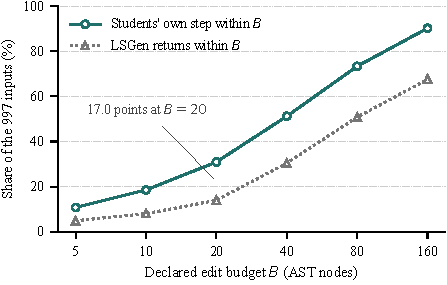
\includegraphics{output/icse-seet-student-reach.pdf}
\caption{Students' own steps and \textsc{LSGen}'s returns within each budget}
\label{fig:reach}
\end{figure}

Our key observation is that solution-supervised repair does not return a step from where the student stands. A return that replaces most of \(b\) is not a continuation of it. Locating a student's regions takes measurement of its own (Section~\ref{sec:introduction}), so we count how much of \(b\) the return keeps. We measure it by the \(\mathrm{ted}^{\dagger}\) of Algorithm~\ref{alg:generic} and by token retention (Section~\ref{sec:experiment}). More precisely, we call a return whose distance from \(b\) is at most a declared budget \(B\) a \emph{bounded step}, where \(B\) is the amount of a student's program a course is willing to give up to one repair.

Figure~\ref{fig:reach} measures how large a step the students themselves take and what \textsc{LSGen} repairs within it, over the 997 Seen inputs. On Seen the 2,581 steps with a defined distance have a median of 15, and one step leaves a median of 96.1\% of the submission's tokens in place. Unrestricted, the returns of \textsc{LSGen} sit at 88.27 and those of the zero-shot model at 27.25. We call the largest step a student took unaided on a problem their \emph{demonstrated reach}. Its median is 39, with quartiles at 15 and 83. An average \textsc{LSGen} return is 2.5 times an average student step and larger than the biggest step the median student took alone. Twenty AST edit operations is close to the median student step and within the demonstrated reach of 30.9\% of students, where \textsc{LSGen} repairs 13.9\%, and 160 covers the demonstrated reach of 90.3\% of students. Surprisingly, four out of five of the submissions \textsc{LSGen} can repair are not repaired within one step, since it repairs 80.2\% of them when nothing bounds the step. This measurement counts what a student changes at once, not which steps lay inside that student's region.

Prior techniques already ask for a small change: \textsc{Refactory} synthesizes minimal repairs~\cite{hu2019re} and \textsc{LSGen} instructs the model to make minimal changes~\cite{dai2026learner}. One alternative is to bound the step of an existing technique. The 13.9\% above is that alternative, and it costs \textsc{LSGen} 66.3 of its 80.2 points, because a generator steered toward an accepted solution has no smaller candidate to fall back on. Returning a hint sidesteps the budget, but the student still has to write the step, and the hint is still fitted to a solution space~\cite{rivers2017data,price2017isnap,roest2024next}. Another alternative is to swap the target for the student's own later submission and leave everything else alone. That is not a one-variable intervention: the same trajectories yield 40,454 Answer examples but 16,973 and 21,416 under Strict and Progress, and the source frequencies move too. What a rule retains moves with it too: among three wrong-answer submissions with pass vectors \((1,0,0)\), \((1,1,0)\), and \((0,1,1)\), verdict-only filtering cannot tell the second from the third, while test-wise progress retains the second, which keeps every passed test and gains one, and not the third, which gains one but loses another. Extra candidates also raise the repair rate on their own: three fixed draws alone account for 15.1 points (Section~\ref{sec:experiment}), so a comparison that does not hold the candidate budget fixed credits the target with them~\cite{zhang2024pydex,koutcheme2024benchmarking,yang2024cref,orvalho2025counterexample,dai2026learner}.

These limitations motivate our approach, which repairs under the guidance of the student's own trajectory. The goal of this paper is to repair a buggy program into one that passes the tests while keeping as much of the submission as possible. In terms of Algorithm~\ref{alg:generic}, we train the generator toward the student's own later submission rather than toward an accepted solution or a solution space. A later submission is a program the student actually produced, so it is reachable by construction; we use it as a preference and let the tests decide what is returned. Our work thus tackles two challenges, (1) that the student's later submission marks the next step only coarsely and may itself be accepted, and (2) that attributing a gain to the target requires holding the sources, the example counts, and the candidate budget fixed.

\begin{figure}[h]
\centering
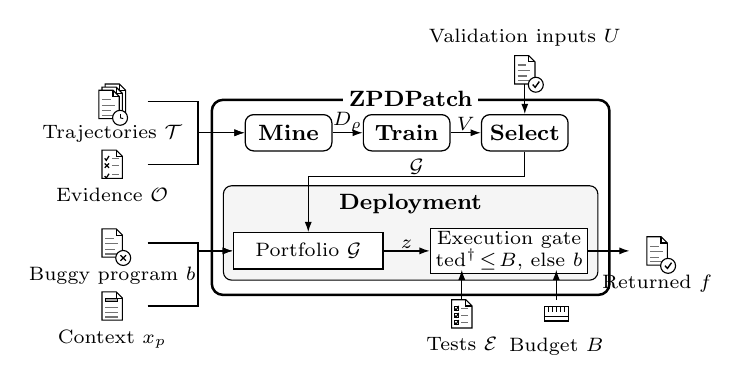
\begin{tikzpicture}[font=\scriptsize, >={Latex[length=1.3mm,width=0.9mm]}, line width=0.45pt,
 stage/.style={draw, rounded corners=3pt, minimum width=11mm, minimum height=4.6mm, align=center,
               font=\footnotesize\bfseries, fill=white, inner sep=1pt},
 sub/.style={draw, minimum width=19mm, minimum height=4.6mm, inner sep=1pt, align=center, fill=white},
 lbl/.style={font=\scriptsize, inner sep=0.5pt},
 item/.style={align=center, inner sep=0.4pt, font=\scriptsize},
 icsheet/.pic={\draw[fill=white, line width=0.4pt]
               (-1.3mm,-1.8mm) -- (-1.3mm,1.8mm) -- (0.5mm,1.8mm) -- (1.3mm,1.0mm) -- (1.3mm,-1.8mm) -- cycle;
             \draw[line width=0.4pt] (0.5mm,1.8mm) -- (0.5mm,1.0mm) -- (1.3mm,1.0mm);},
 iccode/.pic={\pic{icsheet};
            \foreach \y/\a/\b in {0.6/-0.9/0.2, -0.1/-0.9/0.7, -0.8/-0.9/0.3, -1.4/-0.9/0.8}
              \draw[line width=0.42pt, black!55] (\a mm,\y mm) -- (\b mm,\y mm);},
 icstack/.pic={\pic at (0.4mm,0.4mm) {icsheet}; \pic at (0mm,0mm) {icsheet}; \pic at (-0.4mm,-0.4mm) {iccode};},
 icbadge/.pic={\draw[fill=white, line width=0.4pt] (0,0) circle (0.95mm);},
 icclock/.pic={\pic{icbadge}; \draw[line width=0.35pt] (0,0) -- (0,0.45mm); \draw[line width=0.35pt] (0,0) -- (0.4mm,-0.1mm);},
 iccross/.pic={\pic{icbadge}; \draw[line width=0.45pt] (-0.35mm,-0.35mm) -- (0.35mm,0.35mm) (-0.35mm,0.35mm) -- (0.35mm,-0.35mm);},
 ictick/.pic={\pic{icbadge}; \draw[line width=0.5pt] (-0.4mm,0.02mm) -- (-0.08mm,-0.32mm) -- (0.44mm,0.4mm);},
 ichead/.pic={\pic{icsheet};
            \draw[fill=black!35, line width=0pt] (-0.9mm,0.55mm) rectangle (0.7mm,1.0mm);
            \foreach \y in {-0.2,-0.8,-1.4} \draw[line width=0.42pt, black!55] (-0.9mm,\y mm) -- (0.7mm,\y mm);},
 iclist/.pic={\pic{icsheet};
            \foreach \y in {0.7,-0.2,-1.1} {
              \draw[line width=0.33pt] (-0.95mm,\y mm-0.28mm) rectangle (-0.45mm,\y mm+0.28mm);
              \draw[line width=0.4pt] (-0.9mm,\y mm) -- (-0.72mm,\y mm-0.22mm) -- (-0.4mm,\y mm+0.32mm);
              \draw[line width=0.42pt, black!55] (-0.05mm,\y mm) -- (0.85mm,\y mm);}},
 iclog/.pic={\pic{icsheet};
            \draw[line width=0.45pt] (-0.95mm,0.75mm) -- (-0.75mm,0.5mm) -- (-0.4mm,1.05mm);
            \draw[line width=0.45pt] (-0.95mm,-0.45mm) -- (-0.4mm,0.1mm) (-0.95mm,0.1mm) -- (-0.4mm,-0.45mm);
            \draw[line width=0.45pt] (-0.95mm,-1.5mm) -- (-0.75mm,-1.75mm) -- (-0.4mm,-1.2mm);
            \foreach \y in {0.75,-0.2,-1.35} \draw[line width=0.42pt, black!55] (-0.05mm,\y mm) -- (0.85mm,\y mm);},
 icruler/.pic={\draw[fill=white, line width=0.4pt] (-1.5mm,-0.9mm) rectangle (1.5mm,0.9mm);
            \foreach \x in {-1.0,-0.5,0,0.5,1.0} \draw[line width=0.35pt] (\x mm,0.9mm) -- (\x mm,0.25mm);
            \draw[line width=0.35pt] (-1.5mm,-0.35mm) -- (1.5mm,-0.35mm);},
 ictraj/.pic={\pic{icstack}; \pic at (1.0mm,-2.1mm) {icclock};},
 icbuggy/.pic={\pic{iccode}; \pic at (1.4mm,-1.9mm) {iccross};},
 icfixed/.pic={\pic{iccode}; \pic at (1.4mm,-1.9mm) {ictick};}]

 % ---- bands
 \node[stage] (mine)  at (2.80,  5mm) {Mine};
 \node[stage] (train) at (4.30,  5mm) {Train};
 \node[stage] (sel)   at (5.80,  5mm) {Select};
 \node[sub] (gen)  at (3.05, -10mm) {Portfolio $\mathcal G$};
 \node[sub, minimum width=20mm] (gate) at (5.60, -10mm) {Execution gate\\$\mathrm{ted}^{\dagger}\!\le\!B$, else $b$};
 \node[font=\footnotesize\bfseries, inner sep=0.4pt] (dtitle) at (4.35, -4mm) {Deployment};
 \begin{scope}[on background layer]
   \node[draw, rounded corners=3pt, fit=(dtitle)(gen)(gate), inner xsep=1.2mm, inner ysep=0.8mm, fill=black!4] (dep) {};
 \end{scope}
 \begin{scope}[on background layer]
   \node[draw, line width=0.9pt, rounded corners=4pt, fit=(mine)(sel)(dep), inner xsep=1.4mm, inner ysep=1.8mm] (tool) {};
 \end{scope}
 \node[fill=white, inner xsep=2pt, inner ysep=0.4pt, font=\footnotesize\bfseries] at (tool.north) {\textsc{ZPDPatch}};

 % ---- one icon per named item
 \pic at (0.56,  9mm) {ictraj};   \node[item, anchor=north] at (0.56,  6.2mm) {Trajectories $\mathcal T$};
 \pic at (0.56,  1mm) {iclog};    \node[item, anchor=north] at (0.56, -1.8mm) {Evidence $\mathcal O$};
 \pic at (0.56, -9mm) {icbuggy};  \node[item, anchor=north] at (0.56,-11.8mm) {Buggy program $b$};
 \pic at (0.56,-17mm) {ichead};   \node[item, anchor=north] at (0.56,-19.8mm) {Context $x_p$};
 \pic at (5.80, 13mm) {icfixed}; \node[item, anchor=south] at (5.80, 15.8mm) {Validation inputs $U$};
 \pic at (5.00,-18mm) {iclist};  \node[item, anchor=north] at (5.00,-20.8mm) {Tests $\mathcal E$};
 \pic at (6.20,-18mm) {icruler}; \node[item, anchor=north] at (6.20,-20.8mm) {Budget $B$};
 \pic at (7.48,-10mm) {icfixed}; \node[item, anchor=north] at (7.48,-12.8mm) {Returned $f$};

 % ---- wires
 \coordinate (bus) at (1.65, 0);
 \coordinate (corr) at (0, -0.6mm);
 \draw[->] (1.01,  9mm) -- (1.65,  9mm) |- (mine.west);
 \draw[->] (1.01,  1mm) -- (1.65,  1mm) |- (mine.west);
 \draw[->] (1.01, -9mm) -- (1.65, -9mm) |- (gen.west);
 \draw[->] (1.01,-17mm) -- (1.65,-17mm) |- (gen.west);
 \draw[->] (5.80, 11.2mm) -- (sel.north);
 \draw[->] (5.00,-16.2mm) -- (5.00,-12.4mm);
 \draw[->] (6.20,-16.2mm) -- (6.20,-12.4mm);
 \draw[->] (mine) -- node[lbl, above] {$D_\rho$} (train);
 \draw[->] (train) -- node[lbl, above] {$V$} (sel);
 \draw[->] (sel.south) -- (sel.south |- corr) -- node[lbl, above] {$\mathcal G$} (gen.north |- corr) -- (gen.north);
 \draw[->] (gen) -- node[lbl, above] {$z$} (gate);
 \draw[->] (gate.east) -- (7.13, -10mm);
\end{tikzpicture}
\caption{Overview of \textsc{ZPDPatch}}
\label{fig:overview}
\end{figure}

\begin{figure*}[t]
\centering\scriptsize
\begin{minipage}[t]{0.315\textwidth}
\textbf{(a) Buggy submission $b$}\par
\begin{tabular}{@{}r@{~}l@{}}
{\color{black!55}1} & \makebox[4.3cm][l]{\texttt{N~=~int(input())}} \\
{\color{black!55}2} & \makebox[4.3cm][l]{\texttt{for~i~in~range(N):}} \\
{\color{black!55}3} & \colorbox{black!10}{\makebox[4.3cm][l]{\texttt{~~~~if~i**2~>~N:}}} \\
{\color{black!55}4} & \makebox[4.3cm][l]{\texttt{~~~~~~~~print((i-1)**2)}} \\
{\color{black!55}5} & \makebox[4.3cm][l]{\texttt{~~~~~~~~exit()}} \\
\end{tabular}
\end{minipage}\hfill
\begin{minipage}[t]{0.315\textwidth}
\textbf{(b) Progress target: the next submission}\par
\begin{tabular}{@{}r@{~}l@{}}
{\color{black!55}1} & \makebox[4.3cm][l]{\texttt{N~=~int(input())}} \\
{\color{black!55}2} & \makebox[4.3cm][l]{\texttt{for~i~in~range(N):}} \\
{\color{black!55}3} & \colorbox{black!10}{\makebox[4.3cm][l]{\texttt{~~~~if~i**2~>=~N:}}} \\
{\color{black!55}4} & \makebox[4.3cm][l]{\texttt{~~~~~~~~print((i-1)**2)}} \\
{\color{black!55}5} & \makebox[4.3cm][l]{\texttt{~~~~~~~~exit()}} \\
\end{tabular}
\end{minipage}\hfill
\begin{minipage}[t]{0.315\textwidth}
\textbf{(c) Answer target: the accepted submission}\par
\begin{tabular}{@{}r@{~}l@{}}
{\color{black!55}1} & \makebox[4.3cm][l]{\texttt{n~=~int(input())}} \\
{\color{black!55}2} & \colorbox{black!10}{\makebox[4.3cm][l]{\texttt{ans~=~0}}} \\
{\color{black!55}3} & \colorbox{black!10}{\makebox[4.3cm][l]{\texttt{for~a~in~range(10**5~+~1):}}} \\
{\color{black!55}4} & \colorbox{black!10}{\makebox[4.3cm][l]{\texttt{~~~~if~a**2~<=~n:}}} \\
{\color{black!55}5} & \colorbox{black!10}{\makebox[4.3cm][l]{\texttt{~~~~~~~~ans~=~max(ans,~a**2)}}} \\
{\color{black!55}6} & \makebox[4.3cm][l]{\texttt{print(ans)}} \\
\end{tabular}
\end{minipage}
\caption{Running example (p03556), blank lines omitted}
\label{fig:example}
\end{figure*}

\section{Our Approach}
\label{sec:approach}

\subsection{Overview}

\begin{algorithm}[h]
\caption{\textsc{ZPDPatch}}
\label{alg:construct}
\footnotesize
\begin{algorithmic}[1]
\item[\textbf{Input:}] Trajectories ($\mathcal T$), Execution evidence ($\mathcal O$), Validation inputs ($U$), Seeds ($\Sigma$), Portfolio size ($\eta_k$), Edit budget ($B$)
\item[\textbf{Output:}] Portfolio ($\mathcal G$)
\Procedure{ZPDPatch}{$\mathcal T, \mathcal O, U, \Sigma, \eta_k, B$}
 \Statex\hspace{\algorithmicindent}\textit{/* Stage 1. Mine */}
\State $(D_A,D_S,D_P)\gets(\emptyset,\emptyset,\emptyset)$
\For{$\tau=[s_1,\ldots,s_n]\in\mathcal T$}
 \State $D_A\gets D_A\cup\mathsf{TerminalPairs}(\tau)$ \Comment{Answer}
 \For{$\rho\in\{S,P\}$}
  \State $H\gets[s_1]$ \Comment{retained prefix}
  \For{$s_t\in[s_2,\ldots,s_n]$}
   \If{$\mathsf{Improves}_{\rho}(H[-1],s_t;\mathcal O)$}
    \State $D_\rho\gets D_\rho\cup\{(H,c_t)\}$; $H\gets H\mathbin{\|}[s_t]$
   \EndIf
  \EndFor
 \EndFor
\EndFor
 \Statex\hspace{\algorithmicindent}\textit{/* Stage 2. Train */}
\State $V\gets\emptyset$
\For{$(\rho,\sigma)\in\{A,S,P\}\times\Sigma$}
 \State $V\gets V\cup\{\mathsf{Train}(D_\rho,\sigma)\}$
\EndFor
 \Statex\hspace{\algorithmicindent}\textit{/* Stage 3. Select */}
\For{$g\in V$}
 \State $R_g^B\gets\mathsf{Validate}(g,U,B)$ \Comment{$R_g^B\subseteq U$}
\EndFor
\State $\mathcal G\gets\mathsf{Select}(\{R_g^B\}_{g\in V},\eta_k)$ \Comment{$\eta_k=3$}
\State \Return $\mathsf{FreezeAndOrder}(\mathcal G)$
\EndProcedure
\end{algorithmic}
\end{algorithm}

Figure~\ref{fig:overview} illustrates how \textsc{ZPDPatch} repairs a buggy program under the guidance of the student's own trajectory. \textsc{ZPDPatch} takes the inputs of Algorithm~\ref{alg:generic}, namely the buggy program \(b\), the context \(x_p\), and the test suite \(\mathcal E\), together with the trajectories \(\mathcal T\) of a training corpus and their execution evidence \(\mathcal O\). It processes these inputs in the three stages of Algorithm~\ref{alg:construct}, namely Mine, Train, and Select. The Mine stage pairs each buggy submission of a \(\tau\in\mathcal T\), or a retained prefix of it, with a later submission under three target rules, yielding one dataset per rule (Section~\ref{sec:mine}). The Train stage trains one adapter per rule and seed, giving a pool of checkpoints (Section~\ref{sec:train}). The Select stage runs each checkpoint on validation inputs and freezes the \emph{portfolio}, the ordered checkpoints whose executed repairs cover the most of them (Section~\ref{sec:select}). At deployment the portfolio is the generator set \(\mathcal G\) of Algorithm~\ref{alg:generic}, which returns the first candidate that passes every test and otherwise returns the submission unchanged.

\textsc{ZPDPatch} differs from existing techniques in where it obtains the target and in what it holds fixed around it. First, the target is the student's own later submission. Existing techniques supervise the generator toward an accepted solution~\cite{gulwani2018automated,wang2018search,hu2019re}, a solution space built from past correct programs~\cite{piech2015embeddings,rivers2017data,price2017isnap}, or a retrieved learner-specific solution~\cite{dai2026learner}, so what a return aims at is settled without the student's own evidence; the target of \textsc{ZPDPatch} is the next state of the same trajectory that execution evidence shows to be an improvement. Second, because swapping the target also moves the training population and the candidate budget (Section~\ref{sec:limitation}), \textsc{ZPDPatch} holds the sources, the example counts, and the candidate budget fixed across rules and admits a matched-peer target as a control, so a difference in outcome can be read as the target's. The three stages run once per corpus, and deployment issues at most one call per selected checkpoint, so the deployed budget is three calls.

\subsection{\textup{\textsc{ZPDPatch}}}

Algorithm~\ref{alg:construct} details how \textsc{ZPDPatch} instantiates Algorithm~\ref{alg:generic}. Taking \(\mathcal T\) and \(\mathcal O\) in addition to the inputs of Algorithm~\ref{alg:generic}, it builds the generator set offline and requires no instructor solution, no pool of reference programs, and no learner model.

At lines~2--9, Mine scans each trajectory \(\tau\) and emits the pairs of each rule (Section~\ref{sec:mine}). The Answer rule pairs every non-accepted state with the accepted endpoint (line~4), whereas the Strict and Progress rules carry a retained prefix \(H\) and append a state only when the rule's improvement predicate holds on the execution evidence \(\mathcal O\) (lines~7--9), emitting \((H,c_t)\) before the state is appended. At lines~10--12, Train fits one adapter per rule and seed, so the pool \(V\) holds \(|\Sigma|\) checkpoints per rule (Section~\ref{sec:train}). At lines~13--16, Select runs each checkpoint on the validation inputs \(U\) under the edit budget \(B\), records the inputs it repairs, and freezes the portfolio whose union covers the most of \(U\), where \(\eta_k=3\) in our experiments (Section~\ref{sec:select}). Choosing by executed validation repairs rather than by training loss ties the choice to the only outcome a deployment can observe. The returned portfolio \(\mathcal G\) is what line~3 of Algorithm~\ref{alg:generic} iterates over at deployment.

The order of \(\mathcal G\) affects which passing program a student receives, not whether one is found, because every checkpoint of \(\mathcal G\) is invoked until a candidate passes and the gate returns \(b\) unchanged when none does. Hence, given deterministic test outcomes, the repair set of the portfolio contains that of each of its members.


\subsection{Mine}
\label{sec:mine}

The goal of the Mine stage is to make every supervision pair traceable to an observed source and a later submission (lines~2--9). Figure~\ref{fig:example} shows what that choice changes on one trajectory: the Progress target (b) is one Abstract Syntax Tree (AST) edit operation from (a), while the Answer target (c) is 33 operations away and takes another approach. Submissions are grouped by problem and user, chronologically ordered, and cut at the first acceptance. Canonical normalization removes consecutive duplicates while preserving the source code used for generation and execution. A whole-trajectory filter instead excludes a trajectory before splitting if any required prompt--target configuration exceeds 4,096 tokens. Exclusion changes the evaluated population, but never truncates a program or history.

The coarse severity function assigns 0 to Accepted (AC), 1 to Wrong Answer (WA), 2 to Time or Memory Limit Exceeded (TLE/MLE), 3 to Runtime Error (RE), and 4 to Compile Error (CE); unrecognized and internal outcomes occupy the most severe category. Strict compares recorded verdicts. Progress additionally compares replayed outcomes when the recorded verdict strings agree. Its cache must be complete, and compared vectors must have equal, nonempty testcase keys.

For equal testcase universes, \(o_t\prec_\times o_r\) holds when every test in \(o_t\) has severity no greater than its counterpart in \(o_r\), with a strict decrease on at least one. Formally, the improvement predicates are:
\begin{equation}
\begin{aligned}
\mathsf{Improves}_S(r,t)&\iff \mathrm{sev}(v_t)<\mathrm{sev}(v_r),\\
\mathsf{Improves}_P(r,t)&\iff \mathsf{Improves}_S(r,t)\\
 &\quad\lor\ (v_t=v_r\land o_t\prec_\times o_r).
\end{aligned}
\label{eq:progress}
\end{equation}
Intuitively, Equation~\eqref{eq:progress} retains coarse improvements and progress hidden by an unchanged verdict. A severity improvement such as RE to WA need not increase the pass fraction, and a verdict-improving edge does not require test-wise dominance.

Answer emits an independent pair for each non-AC source and the accepted endpoint. Thus \([s_1,\ldots,s_9]\) yields \(([s_1],c_9),\ldots,([s_8],c_9)\); it does not expose accumulated prefixes to Answer training. Strict and Progress start with \(H=[s_1]\), compare each later state with the \emph{last retained} state, and append it only when the predicate holds. Before appending \(s_t\), the builder emits \((H,c_t)\). For WA, improved WA, AC, Strict emits \(([s_1],c_3)\), whereas Progress emits \(([s_1],c_2)\) and \(([s_1,s_2],c_3)\). The accepted endpoint remains eligible in both rules. Although Strict's pairwise predicate is contained in Progress's, their independently scanned edge sets need not be nested.

Chronological indices strictly increase, so construction terminates without cycles. With fixed-key evidence, retained edges also decrease the appropriate verdict/test severity rank. These are builder invariants, not evidence of a learned ZPD effect. Binary accepted/non-accepted mining retains 14,027 of 16,973 Strict pairs and 18,009 of 21,416 Progress pairs. Models retrained on them agree with the canonical ones on 84.6\% and 87.5\% of Seen repair decisions (Section~\ref{sec:generality}), so we read the ranking as operational rather than universal.

\subsection{Train}
\label{sec:train}
The goal of the Train stage is to learn each rule independently while keeping model and optimization comparable (lines~10--12). The implementation fine-tunes Qwen2.5-Coder-7B-Instruct with 4-bit Quantized Low-Rank Adaptation (QLoRA)~\cite{hui2024qwen2,dettmers2023qlora}. Adapters have rank 16, scaling 32, and dropout 0.05, targeting attention and feed-forward projections. Canonical training uses one epoch, learning rate \(2\times10^{-4}\), and seeds 2027--2029. Assistant target tokens supply cross-entropy loss. The role-neutral prompt contains the statement, limits, permitted submissions, execution/edit summaries, and a request for a complete solution. It names neither the rule nor a preferred patch size, so specialization must come from the data rather than explicit instructions.

Targets are future submissions available offline; inference inputs contain only observed states. Current-only controls reset positions and remove earlier entries, preventing length leakage through position labels. Answer training is already single-source, so supplying history at inference creates a distribution change. The history-removal retraining control instead holds targets fixed and changes earlier-submission serialization. Source-matched target training holds current input and count fixed.

The paired-target control inner-joins records by problem, user, submission identifier, and the exact buggy program, retaining sources with distinct Answer and Progress targets. Its 7,389 training and 931 validation examples per condition use identical current-only inputs. The separate peer control requires another user on the same problem and in the same split, with exactly equal target execution evidence. Writing \(y_u\) for the same-user target and \(y'\) for its peer replacement, for semantic-token diff distance \(d\) the discrepancy \(\delta=|d(c,y')-d(c,y_u)|\) must satisfy \(\delta\le2\) or \(\delta/\max(1,d(c,y_u))\le0.1\). Scarce evidence groups are visited first; ties prioritize distance discrepancy, reuse, and identifier, with donor reuse capped at three. This greedy rule yields 5,231 training and 306 validation examples per condition. Equal outcomes and nearby distances do not equate structure or style, so its measured effect belongs to the entire replacement rule, not isolated provenance.

\subsection{Select}
\label{sec:select}
The goal of the Select stage is to deploy a bounded portfolio chosen without final-test outcomes (lines~13--16). For validation inputs \(U\), let \(R_g^B\) be inputs repaired by checkpoint \(g\) within edit budget \(B\). Formally, selection maximizes:
\begin{equation}
 J_B(\mathcal G)=\frac{1}{|U|}\left|\bigcup_{g\in\mathcal G} R_g^B\right|,\qquad |\mathcal G|=3.
\label{eq:portfolio}
\end{equation}
Intuitively, Equation~\eqref{eq:portfolio} rewards complementary successes, not low training loss or the presence of every rule. Validation uses one fixed-hash trajectory from each of 461 eligible problems. The mixed pool has nine checkpoints and 84 candidate portfolios; requiring one checkpoint per rule instead permits 27. The primary unconstrained mixed choice is Answer2027, Answer2028, and Progress2027. The rule-constrained choice is a different condition. Answer-9Choose3 receives nine Answer checkpoints and the same search over 84 portfolios. Ties use recorded pass-rate, improvement, and deterministic identifier priorities. Budget-indexed selection repeats the declared objective at \(B\in\{5,10,20,40,80,160\}\), without choosing a budget from test results.

Selected checkpoints and order are frozen. Each emits at most one independent candidate, and the first observed acceptance stops generation. If none passes all tests, Algorithm~\ref{alg:generic} prioritizes pass fraction and then smaller distance. Because unchanged code is feasible, for the same fixed execution measurements the returned pass fraction cannot decrease, and a finite edit budget cannot be exceeded. This is not per-test non-regression: equal fractions can conceal gains and losses on different tests. It also does not guarantee non-regression under fresh execution, an unseen suite, or resource variability.

Terminal pairing is linear in trajectory length; replaying \(n\) submissions on \(m\) tests requires \(O(nm)\) executions and evidence storage. The search over 84 portfolios is bounded at our pool size, not a scalable optimizer.

\section{Experiments}
\label{sec:experiment}
In this section, we evaluate \textsc{ZPDPatch} to answer the following research questions:
\begin{itemize}
\item RQ1: How effectively does \textsc{ZPDPatch} repair buggy submissions?
\item RQ2: How does the target rule change what a repair keeps of the student's program?
\item RQ3: What do candidate breadth, checkpoint identity, and serialized history contribute?
\item RQ4: Which findings replicate across problems, prefixes, model scales, and a classroom corpus?
\end{itemize}
We implemented \textsc{ZPDPatch} on top of Qwen2.5-Coder-7B-Instruct~\cite{hui2024qwen2}, an open code model of a scale a course can host. All experiments were conducted on a single machine equipped with one NVIDIA RTX 5090.

\subsection{Experimental Settings}


\begin{table}[t]
\caption{Corpus after whole-trajectory filtering}
\label{tab:data}
\centering\scriptsize\setlength{\tabcolsep}{2.5pt}
\begin{tabular}{ll||rrrrrr}
\toprule
Group & Part. & Probl. & Tests & Traj. & Subm. & Prefixes & Users \\
\midrule
\multirow{3}{*}{Seen} & Train & 492 & 9,446 & 14,027 & 54,481 & 40,454 & 4,012 \\
 & Valid & 492 & 9,446 & 1,754 & 6,719 & 4,965 & 1,248 \\
 & Test & 492 & 9,446 & 1,754 & 6,598 & 4,844 & 1,250 \\
Unseen & Test & 54 & 642 & 259 & 954 & 695 & 236 \\
\midrule
Total & & 546 & 10,088 & 17,794 & 68,752 & 50,958 & -- \\
\bottomrule
\end{tabular}
\end{table}

\noindent\textbf{Baselines.} Zero-shot uses the same base model without fine-tuning and appends verdict/pass-count feedback after failure. \textsc{LSGen} retains repair-pair filtering, edit-vector retrieval, diff-guided generation, and re-retrieval~\cite{dai2026learner}; its same-problem Seen-Train references are unavailable under our Unseen information constraint, so that condition is not evaluated. Answer-1 uses one Answer checkpoint. Answer-3Seed uses seeds 2027--2029 on the same 40,454 Answer pairs. Answer-9Choose3 adds seeds 2030--2035 and selects three from nine. Mixed-9Choose3 denotes the primary unconstrained \textsc{ZPDPatch} pool.

\noindent\textbf{Benchmarks.} Table~\ref{tab:data} describes the Project CodeNet Python800 corpus~\cite{puri2021codenet} by partition (Part.) and submissions (Subm.); its Seen problems and tests are shared across partitions, so the user counts are not additive. We retain trajectories with at least three submissions, a non-AC state before the first acceptance, and an accepted endpoint in the benchmark reference set. Whole-trajectory 4,096-token filtering removes 3,660 trajectories before splitting. Problems ranked by eligible trajectory count supply the top 90\% to Seen (492) and the remaining 54 to Unseen; Seen trajectories are split 80:10:10 within every problem. The primary endpoint is the last recorded non-AC submission of an eventually successful trajectory, and runtime eligibility requires the buggy program to remain non-AC and the recorded accepted endpoint to pass the available tests on replay. This leaves 997 of 1,754 Seen test trajectories, from 328 problems, and 250 of 259 Unseen trajectories, from all 54 problems; excluded trajectories do not enter the denominator. CodeNet users are online-judge participants, not a verified classroom population. We also use TIKTOC's~\cite{duan2024tiktoc} release of authentic Java CodeWorkout submissions and tests from an Introductory Programming (CS1) course: 1,125 trajectories from 224 students and 17 exercises, with 181 test trajectories from 33 held-out students. CodeWorkout is a practice platform where a course assigns short method-level exercises with instructor-authored tests. A separate exercise split has 10/3/4 train/validation/test exercises and 605/216/304 trajectories.

\begin{table}[h]
\caption{Primary Python evaluation. H: history input; C: current-only}
\label{tab:main}
\centering\small
\begin{tabular}{@{}ll||rr|rr@{}}
\toprule
Method & Input & \multicolumn{2}{c|}{Seen} & \multicolumn{2}{c}{Unseen} \\
 & & RR (\%) & TED & RR (\%) & TED \\
\midrule
Zero-shot & H & 30.7 & 27.25 & 62.0 & 17.46 \\
\textsc{LSGen} & H & 80.2 & 88.27 & -- & -- \\
Answer-1 & C & 58.1 & 30.27 & 69.6 & 15.30 \\
Answer-3Seed & H & 61.7 & 24.52 & 73.2 & 13.38 \\
Answer-9Choose3 & H & 59.8 & 25.46 & 74.8 & 15.19 \\
Mixed-9Choose3 & H & 61.5 & 21.05 & 74.8 & 11.40 \\
\midrule
Answer-3Seed & C & 72.0 & 37.94 & 81.2 & 16.01 \\
Answer-9Choose3 & C & 69.5 & 35.41 & 82.0 & 20.06 \\
\bottomrule
\end{tabular}
\end{table}

\noindent\textbf{Evaluation Metrics.} We measure three kinds of outcome: whether the returned program passes the tests, how large its change is, and how much of the submission it keeps. \emph{Repair Rate} (RR) is the fraction of eligible inputs whose returned program passes every test. Tree Edit Distance (TED) between ASTs measures current-to-returned change~\cite{zhang1989simple,pawlik2016tree} and is undefined when either program does not parse. Undefined cases remain in unrestricted RR but not in TED summaries, and finite gates reject undefined-distance changes. Unpaired TED averages successful, parseable returns, while paired locality uses joint successes. \emph{Retention} divides tokens or nonempty stripped lines matched by \texttt{SequenceMatcher} by the source count. Unless stated otherwise, brackets give 95\% percentile bootstrap intervals over problem clusters~\cite{efron1979bootstrap,wilson1927probable}, Java resamples students and exercises separately, and equal-problem estimates average problem means. McNemar tests are supplementary to those intervals~\cite{mcnemar1947note}, and Holm adjustment covers the history-removal retraining tests~\cite{holm1979simple}.


\subsection{RQ1: Repair Effectiveness}
\label{sec:rq-effectiveness}

\begin{figure}[t]
\centering
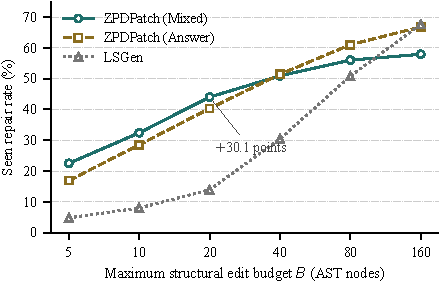
\includegraphics{output/fse2027-budget-frontier.pdf}
\caption{Seen repair rate at each declared edit budget}
\label{fig:budget}
\end{figure}

\begin{table}[h]
\caption{Source- and count-matched target replacement}
\label{tab:targets}
\centering\small
\begin{tabular}{l||rr|rr}
\toprule
Population & \multicolumn{2}{c|}{RR (\%)} & \multicolumn{2}{c}{Retention (pp)} \\
 & Answer & Progress & Tokens & Lines \\
\midrule
Seen (997) & 53.2 & 34.0 & +5.6 & +8.9 \\
Unseen (250) & 76.8 & 65.6 & +6.5 & +10.4 \\
Java (181) & 85.6 & 50.8 & +4.8 & +5.1 \\
\bottomrule
\end{tabular}
\end{table}
RQ1 asks how effectively \textsc{ZPDPatch} repairs buggy submissions. To this end, we compared every configuration and baseline on the same inputs, both unrestricted and under a declared edit budget. In terms of unrestricted repair rate, Table~\ref{tab:main} identifies current-only Answer-3Seed as the retained deployment configuration within our implementation, at 72.0\% Seen and 81.2\% Unseen. Relative to current-only Answer-1, its paired gain is 13.9 points [11.71, 16.29] and 11.6 points [7.32, 16.23]. RQ3 separates checkpoint identity from opportunity count. Current-only Answer-9Choose3 trades 25 Seen repairs for two Unseen ones (205/250 against 693/997), so we keep the fixed portfolio. Current-only mixed-pool reselection chooses exactly that triple.

\noindent\textbf{Operational locality.} Figure~\ref{fig:budget} gives the repair rate at each declared budget over the 997 Seen inputs. At a budget of 20 AST edit operations, Mixed repairs 44.0\% of Seen inputs versus \textsc{LSGen}'s 13.9\%, a 30.1-point difference [26.45, 33.82]. Across the six prespecified budgets its mean advantage over \textsc{LSGen} is 14.7 points [12.03, 17.43]. The advantage is budget-indexed: \textsc{LSGen} leads again at 160. On Unseen the same order holds through 20 and reverses at 40.

The history-input mixed portfolio repairs 613/997 Seen and 187/250 Unseen inputs. Its Seen gain over Zero-shot is 30.8 points [26.43, 35.09], or 26.1 [21.24, 30.93] with equal problem weights. Mixed-only and Zero-shot-only successes are 342 against 35 (McNemar \(p<10^{-63}\)). This is not a history-specific effect: Mixed nearly ties Answer-3Seed, while its matched nine-checkpoint contrast is +1.7 points [-0.79, 4.29] on Seen and 0.0 [-3.70, 3.75] on Unseen.

\textsc{LSGen} repairs 800/997 Seen inputs versus Mixed's 613/997, a difference of -18.8 points [-23.04, -14.46]; 80 versus 267 exclusive successes give \(p<10^{-23}\). On joint repairs, Mixed's TED is lower by 43.34 [38.47, 48.44] relative to \textsc{LSGen} and 8.46 [5.05, 12.55] relative to Zero-shot. Conditioning excludes unilateral successes, so smaller patches do not cancel the deficit. The cause of that deficit is the search space: \textsc{LSGen} retrieves a learner-specific solution for every input and retrieves again after each failure, whereas our deployment issues three calls from the frozen portfolio. The deficit sits at the unrestricted end, and the order reverses once an edit budget is declared. Overall, the deployed configuration repairs the most within a declared budget and trails \textsc{LSGen} only when nothing bounds the edit, so we retain current-only Answer-3Seed.

\subsection{RQ2: Target Construction and Locality}
\label{sec:rq-locality}

RQ2 asks how the target rule changes what a repair keeps of the student's program. To this end, we replaced the target while holding the sources and the example counts fixed, and repeated the comparison on student-held-out Java.

\noindent\textbf{Matched targets.} Table~\ref{tab:targets} changes the target while holding current inputs and training counts fixed. Progress-minus-Answer RR is -19.2 points [-22.96, -15.54] on Seen and -11.2 [-17.37, -4.88] on Unseen, with exact McNemar \(p=7.85\times10^{-34}\) and \(p=6.17\times10^{-5}\). The Answer dataset's advantage is therefore not only more training records. The intervention is the target rule, not a clean incorrect-versus-correct contrast. Under the matched inputs the Progress rule repairs 34.0\% of Seen inputs and improves 43.4\%, so a further 9.4 points receive a program that advances without passing, against 53.2\% and 65.0\% for the Answer rule. The same two gaps are 6.4 and 7.6 points on Unseen, and 9.4 against 2.2 on Java, where Answer targets already repair 85.6\% outright. Part of the coverage the Progress rule gives up therefore returns as partial progress, counted by test execution and not by comprehension. The cause lies in the target itself: a Progress target is not required to pass, so the generator trained on it returns programs that advance without passing.

Progress's locality benefit is visible on joint successes. Among 299 Seen and 154 Unseen jointly repaired inputs, 278 and 134 have defined source-to-repair TED for both methods. Answer-minus-Progress mean TED is 10.08 [7.53, 12.99] and 6.83 [4.58, 9.39]. Token retention improves by 5.6 [4.29, 6.94] and 6.5 [4.26, 8.95] points; line retention improves by 8.9 [6.64, 11.16] and 10.4 [6.95, 14.25]. The 21 and 20 undefined-TED cases remain in RR and are not declared unrepairable. These measures describe successful outputs that retain more of the submission, not easier comprehension.



\begin{table}[h]
\caption{Java matched-target outcomes over 17 exercises and 90 jointly repaired students}
\label{tab:uneven}
\centering\small
\begin{tabular}{@{}lr||lr@{}}
\toprule
\multicolumn{2}{c||}{Repairs (17 exercises)} & \multicolumn{2}{c}{Retention (90 students)} \\
\midrule
Answer higher & 15 & Answer higher & 5.6\% \\
Tied & 2 & Tied & 63.3\% \\
Progress higher & 0 & Progress higher & 31.1\% \\
Extra Answer repairs & 63 & Median gain & 9.6 \\
Largest gap & 12 & Retention range & -21.1 / 49.7 \\
\bottomrule
\end{tabular}
\end{table}

Java retraining uses 600 training and 118 validation pairs per target. Answer targets repair 155 trajectories and Progress targets 92, a difference of 34.8 points; Progress-minus-Answer intervals are [-44.91, -25.47] under student clustering and [-47.31, -23.79] under exercise clustering. Among 90 joint repairs, Progress targets increase lexical-token retention by 4.8 points and line retention by 5.1 points, with intervals [2.79, 7.19] and [2.92, 7.25]. This is evidence for a coverage--locality tradeoff across two languages and populations.




\begin{figure}[t]
\centering\scriptsize
\begin{minipage}[t]{0.47\columnwidth}
\textbf{(a) Progress repair: 20 of 21 lines kept (TED 1)}\par\smallskip
\begin{tabular}{@{}r@{~}l@{}}
{\color{black!55}1} & \makebox[3.4cm][l]{\texttt{N=int(input())}} \\
{\color{black!55}2} & \makebox[3.4cm][l]{\texttt{S=input()}} \\
{\color{black!55}\smash{$\vdots$}} & \\
{\color{black!55}12} & \colorbox{black!10}{\makebox[3.4cm][l]{\texttt{~~while~j>=0:}}} \\
{\color{black!55}\smash{$\vdots$}} & \\
{\color{black!55}21} & \makebox[3.4cm][l]{\texttt{print(ans)}} \\
\end{tabular}
\end{minipage}\hfill
\begin{minipage}[t]{0.47\columnwidth}
\textbf{(b) Answer repair: 3 of 21 lines kept (TED 83)}\par\smallskip
\begin{tabular}{@{}r@{~}l@{}}
{\color{black!55}1} & \makebox[3.4cm][l]{\texttt{N=int(input())}} \\
{\color{black!55}2} & \makebox[3.4cm][l]{\texttt{S=input()}} \\
{\color{black!55}3} & \colorbox{black!10}{\makebox[3.4cm][l]{\texttt{cnt=S.count('R')}}} \\
{\color{black!55}4} & \colorbox{black!10}{\makebox[3.4cm][l]{\texttt{ans=S[:cnt].count('W')}}} \\
{\color{black!55}5} & \makebox[3.4cm][l]{\texttt{print(ans)}} \\
\end{tabular}
\end{minipage}
\caption{What each rule returns for one jointly repaired submission}
\label{fig:case}
\end{figure}

\begin{figure}[t]
\centering
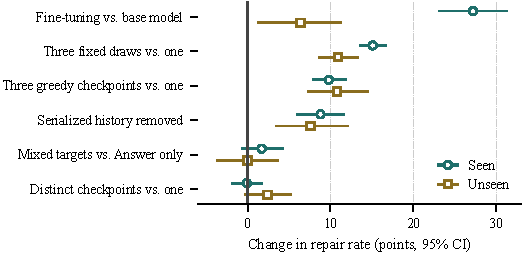
\includegraphics{output/icse-seet-ablation.pdf}
\caption{What each change does to the repair rate}
\label{fig:ablation}
\end{figure}

\noindent\textbf{What a student receives.} Cohort means do not describe an individual student, so Table~\ref{tab:uneven} resolves the Java contrast by exercise and by student. One exercise accounts for 12 of the 63 additional Answer repairs, and there Progress targets repair 3 of 15 trajectories against 15. Most students who receive a working repair from either rule get back the same amount of their own code, about a third get more, by a median of 9.6 points, and a few get less. Line retention behaves the same, zero for 64.4\% of students with maximum 47.6. Figure~\ref{fig:case} illustrates that tail on Python. The student's own preceding edit changed \texttt{i<j} to \texttt{i<=j} and left 93.3\% of the tests passing; the Progress-target repair (a) changes one line more, \texttt{j>0} to \texttt{j>=0}, whereas the Answer-target repair (b) returns a five-line program that keeps three of the student's 21 lines. Both pass every test under the same gate and budget.

\noindent\textbf{Peer targets.} The separate outcome- and distance-matched replacement raises RR from 50.4\% to 54.7\% on Seen and from 78.4\% to 84.4\% on Unseen. Same-minus-peer intervals are [-7.71, -0.84] and [-11.79, -0.41], with exact McNemar \(p=0.005\) and \(p=0.032\). Equal outcomes with nearby distances still permit differences in structure, so the contrast does not isolate user identity. Matched peer targets improve coverage here; one's own trajectory is not uniquely necessary under this control. Overall, target construction moves coverage and locality in opposite directions under matched inputs and in the same direction on student-held-out Java, and the effect is not uniform across exercises or students.

\subsection{RQ3: Component Efficacy}

RQ3 asks what candidate breadth, checkpoint identity, and serialized history each contribute. To this end, we compared controls that change one of them at a time within the stored executions.

\noindent\textbf{Fixed candidate breadth.} Figure~\ref{fig:ablation} reports what each matched control does to the repair rate, with 95\% intervals. For three stored draws with success indicators \(a_{ij}\), the expected uniformly selected one-draw success for input \(i\) is \(\frac{1}{3}\sum_j a_{ij}\), whereas the three-draw union succeeds when \(\max_j a_{ij}=1\). Their paired difference isolates additional opportunities within the identical candidate set. Replacing greedy decoding by one stochastic draw costs 7.6 points [-9.81, -5.41], whereas execution-selecting three of those identical fixed draws contributes 15.1 points [13.48, 16.76] on Seen. It shows why comparing a portfolio only with one adapter overstates the evidence for its training signal.

The temperature sweep retains all declared conditions. Through \(T=1.0\) the one-draw rate stays within 41.1--43.1\% on Seen, the three-draw union reaches 60.0/75.2\%, and at \(T=1.5\) the decoder collapses to 15.8/35.2\%. Fine-tuning also matters: the matched base-model three-draw union reaches only 30.4/65.6\%, so adaptation adds 27.2 points [22.99, 31.41] on Seen and 6.4 points [1.19, 11.34] on Unseen. Breadth alone therefore does not explain all improvement over the base model.

At matched temperature, replacing three draws of one checkpoint by one draw from each of three checkpoints changes RR by -0.1 points [-2.00, 1.80] on Seen and 2.4 points [-0.41, 5.31] on Unseen. These intervals do not establish a consistent advantage from checkpoint diversity. A deterministic multi-seed gain can coexist with this result because sampling from one checkpoint already supplies diversity.

A current-only factorial on one inference stack tests this explanation. Three greedy checkpoints gain 9.8 [7.85, 11.92] and 10.8 [7.23, 14.64] points over one, but under the matched stochastic decoder distinct checkpoints add only 2.1 points [0.00, 4.16] and 1.2 points [-2.93, 5.93], with the equal-problem Seen interval including zero. Because the backend changes the absolute rates, our recommendation covers the stack we evaluated.

\noindent\textbf{Serialized history.} Removing earlier submissions from the frozen portfolios raises repair for both pools. The gains are 8.8/11.1 Seen points and 7.6/6.0 Unseen points for Mixed/Answer, with all intervals excluding zero. Matched retraining without that context shows no significant difference after Holm correction, with smallest adjusted \(p=0.313\), so serialized history is not part of the measured advantage and the deployed configuration uses current-only prompts.

Answer-9Choose3 receives the same nine-checkpoint pool size and 84-subset opportunity as Mixed. The primary five-fold cross-fitted mixed-minus-Answer contrast is +2.2 points [-0.19, 4.63], compared with the non-cross-fitted +1.7 [-0.79, 4.29]. Overall, candidate breadth and adaptation each contribute measured gains, whereas distinct checkpoints add no consistent advantage once the stochastic decoder is matched and serialized history is not supported as a necessary input.

\subsection{RQ4: Generality}

\begin{figure}[t]
\centering
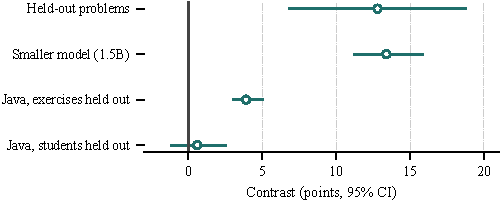
\includegraphics{output/icse-seet-replication.pdf}
\caption{Where the findings replicate}
\label{fig:replication}
\end{figure}
\label{sec:generality}
RQ4 asks which findings replicate across problems, prefixes, model scales, and a classroom corpus. To this end, we measured the same contrasts again on held-out problems, earlier prefixes, a smaller model, and the classroom corpus.

\noindent\textbf{Problems and execution suites.} Figure~\ref{fig:replication} collects the contrast and its interval in each replication setting. Within Unseen, Mixed exceeds Zero-shot by 12.8 points [6.83, 18.75], with 45 versus 13 exclusive successes and exact McNemar \(p=3.01\times10^{-5}\). On the 122 joint repairs with defined TED it reduces TED by 6.41 [3.43, 9.89]. The higher absolute Unseen RR is not evidence of stronger generalization: the partitions differ in availability and composition. Matching all 54 Unseen problems to distinct Seen problems on six pre-repair difficulty covariates changes the raw gap into -4.6 equal-problem points [-14.18, 5.30]. We therefore rely on within-split paired contrasts rather than the raw cross-split difference.

A second check splits the authored suite into an observed slice and a held-back slice. Among the inputs each repairs on the observed slice, 189/192 (98.4\%) and 184/186 (98.9\%) also pass the held-back slice, and 13 versus 8 exclusive joint successes yield \(p=0.383\). Repeating the procedure on all 328 Seen problems with a distinct seed yields 97.8\% and 97.9\% confirmation. These are held-back slices of the same authored tests, so the conditional percentage must not replace the full-denominator repair rate.

\noindent\textbf{Earlier prefixes.} Across 2,770 Seen and 674 Unseen executable prefixes of eventually successful trajectories, current-only Answer-3Seed reaches 69.6\% and 80.1\% RR. The early, middle, and last thirds reach 70.0\%, 67.6\%, and 71.4\% on Seen and 82.9\%, 77.3\%, and 81.8\% on Unseen. Multiple prefixes from one trajectory are dependent, so this rate is not added to the 997-input result.

\noindent\textbf{Model scale and classroom data.} At 1.5B parameters three checkpoints still gain 13.4 points over one [11.16, 15.92], but mixed-minus-Answer is -0.8 [-2.62, 1.07]. Mixed reaches 50.3\% and the nine-checkpoint Answer control 51.1\% on Seen. This smaller model reproduces the utility of multiple opportunities, not an unrestricted mixed-target advantage.

The Java portfolio results differ from RQ2's direct matched-target retraining. Its interval is [2.99, 5.11] on held-out exercises and [-1.20, 2.59] on held-out students. Absolute RR is 56.2\% versus 52.3\% over 304 exercise-held-out trajectories and 84.0\% versus 83.4\% over 181 student-held-out trajectories. The exercise estimate rests on four clusters: refitting with one exercise left out keeps the contrast between 3.6 and 4.4 points, and single exercises range from 2.5 to 5.5 points. Four clusters cannot support a broad classroom-population claim.

\noindent\textbf{Representation and overlap.} Binary accepted/non-accepted mining removes the fine severity ordering but also changes the target set. Retraining changes Progress RR by +2.3 Seen and -2.8 Unseen points in the canonical-minus-alternative direction. Because the changes go in opposite directions, the ordering is not a free implementation choice. For Mixed and Answer-9Choose3, exact matches between a returned repair and a training-time accepted program occur in 0.6\% and 1.3\% of selections, near-duplicates above a 0.90 token-similarity threshold in 3.8\% and 5.3\%, and median maximum similarity to a same-problem training target is 66.7\% and 68.6\%. Low exact-copy rates do not exclude structural reuse or pretraining contamination~\cite{allamanis2019adverse}. Overall, the matched-target tradeoff replicates on student-held-out Java and candidate breadth remains useful at a smaller model scale, whereas mixed-target unrestricted superiority does not replicate consistently.

\subsection{Discussion}

\noindent\textbf{Implications for instructors.} Our results suggest three ways a course can use these repairs. First, declaring an edit budget still leaves repairs to show: within 20 AST edit operations our configuration repairs 44.0\% of the Seen inputs where \textsc{LSGen} repairs 13.9\% (Section~\ref{sec:rq-effectiveness}). Second, which rule a course deploys follows from whether coverage or locality binds, since the Progress rule keeps more of the student's tokens on the inputs both rules fix and repairs fewer of them (Section~\ref{sec:rq-locality}). Third, that choice is better made per exercise than for a whole course, because cost and gain are uneven across exercises and students (Section~\ref{sec:rq-locality}).

\noindent\textbf{Delivering repairs.} A returned program can be shown as it is, reduced to the lines it changed, or passed to a hint generator as input~\cite{phung2023generating,roest2024next}. Since handing a model a solution steers its hints toward that solution, a return that keeps more of the student's own approach is likely the better input for such hints as well.

\subsection{Threats to Validity}
(1) Runtime variability, undefined source ASTs, and Python whitespace affect labels and distances. We retain unknowns, denominators, and whitespace-sensitive corrections, but hashes establish provenance, not correctness, and source and peer matching do not equate all target semantics or styles. (2) Acceptance is not proof of semantic correctness~\cite{smith2015cure}, same-suite slices are not independent specifications, and TED and retention do not measure cognitive load or subsequent learning. CodeNet does not identify novices or measure mastery, Java supplies classroom submissions rather than an intervention observing feedback use, and the per-exercise and per-student resolution describes which students would receive a different repair, not which students benefit, with Figure~\ref{fig:case} one post-hoc case that carries no estimate. We display a CodeNet program because the course data terms do not permit redistributing student submissions. (3) The comparison covers the retrieval-based and model-based lines, not the alignment-based one. Filtering favors short, eventually successful Python trajectories and permits Seen user overlap, Java adds one course context and only four held-out exercises, and cluster bootstrap and equal-problem estimates do not eliminate small-cluster uncertainty, multiplicity, or the bias of analyses chosen after earlier results. These distinctions limit educational and target-quality interpretations.

\section{Related Work}
\label{sec:related}
\noindent\textbf{APR for Programming Assignments.} Generate-and-validate repair spans search, learned transformations, and language models~\cite{gazzola2019automatic,monperrus2018automatic,weimer2009automatically,legoues2012genprog}; search analyses~\cite{qi2014strength} and execution-based evaluation~\cite{haque2023fixeval,chen2021evaluating} separate candidate quality from exposure, and training signals range from neural patches and ensembles to synthetic corruption and self-supervision~\cite{tufano2019empirical,lutellier2020coconut,yasunaga2021break,ye2022selfapr}, including none at all~\cite{xia2022less,jiang2023impact}. Beyond the techniques described in Section~\ref{sec:preliminaries}, many techniques repair student submissions. Among alignment-based techniques, clustering, alignment, and refactoring exploit correct programs of the same problem~\cite{gulwani2018automated,wang2018search,hu2019re}, assignment-aware selection varies which references are used~\cite{heo2023referent,choi2021automated,choi2025automated}, and tutoring systems propagate feedback and generate hints~\cite{piech2015embeddings,glassman2015overcode,rivers2017data,price2017isnap}. Among language-model-based techniques, models support repair, syntax feedback, conversations, peers, and counterexamples~\cite{joshi2023repair,zhang2024pydex,phung2023generating,liu2024fastfixer,yang2024cref,zhao2026peer,orvalho2025counterexample}. We compare against the retrieval-based and language-model-based lines under one information constraint and exclude the others for a reason each: alignment-based techniques align against accepted programs of the same problem, an input our Unseen condition withholds; assignment-aware selection varies that same input; and next-step hint generators return one edit rather than a program, so the gate and the budget of Algorithm~\ref{alg:generic} do not apply. We do not introduce portfolio repair; we isolate trajectory targets with same-target seeds, equal search spaces, fixed draws, and current-only controls.

\noindent\textbf{Feedback on the Student's Own Work.} A second line fits its guidance to a record of student work. Data-driven hints read a solution space or a past cohort's paths and project the submission onto it, so two students at the same position receive the same next step whatever tests their own code passes~\cite{rivers2017data,price2017isnap,roest2024next}; a hint and a program are also measured on different scales~\cite{yi2017feasibility,koutcheme2024benchmarking,keuning2018systematic}. \textsc{LSGen} also mines chronological wrong-to-later-correct submission pairs for retrieval~\cite{dai2026learner}, so trajectories are not our novelty; it does not separate the history's contribution from that of extra candidates, however, which is why we hold both fixed together. ZPD and scaffolding concern supported performance, not program edit distance~\cite{cole1978mind,murray2002toward,chounta2017grey,schulze2024beyond}, knowledge tracing models proficiency from interactions~\cite{corbett1994knowledge,piech2015deep,ghosh2020context}, and TIKTOC incorporates testcase evidence~\cite{duan2024tiktoc}. Next-step hints, feedback ladders, and novice-response studies examine guidance more directly~\cite{roest2024next,heickal2024generating,xiao2024exploring}, while feedback theory emphasizes its interpretation and use~\cite{narciss2008feedback,hattie2007power,shute2008focus,aleven2000limitations}. In contrast, \textsc{ZPDPatch} reads the submission's own execution evidence and returns a complete program whose target is a step the same student later took, so it exposes a coverage--locality tradeoff rather than dominance over feedback strategies. To our knowledge, \textsc{ZPDPatch} is the first repair technique that makes a step from the student's own trajectory the training target rather than a retrieval input. This paper does not claim that a learner's serialized history improves generated repairs: our deployed configuration prompts with the current submission alone, and the supplement reports the controls behind that choice, including their negative outcomes.

\section{Conclusion}
\label{sec:conclusion}
Automated Program Repair has substantially raised the repair rate for buggy student submissions. However, existing techniques settle what a return aims at without reference to the student's own attempts, so a return can replace most of the submission. This paper aims to repair a buggy submission toward a step taken from the student's own trajectory. To this end, \textsc{ZPDPatch} mines supervision pairs from execution evidence, trains one adapter per rule, and freezes a portfolio by executed validation repairs. Experimental results demonstrate the same coverage--locality tradeoff in matched Python and student-held-out Java experiments, uneven across exercises and students, while candidate breadth and model adaptation account for the rest of the improvement. We therefore retain the current-only Answer portfolio and report the Progress rule as the option for when locality binds. We hope that \textsc{ZPDPatch} helps a course return repairs that continue a student's own attempt rather than replace it.

\section*{Data Availability}
An anonymous supplement contains the paired outcomes, condition manifests, metric code, negative results and claim--evidence links; its offline verifier recomputes every reported contrast. Student source and model weights are excluded under the CodeWorkout/TIKTOC~\cite{duan2024tiktoc} and CodeNet~\cite{puri2021codenet} terms, and no student intervention was conducted.


\noindent\textbf{Research process.} OpenAI Codex assisted with design, code, orchestration, diagnostics, and manuscript preparation under author instructions, and automated agents executed authorized jobs; we do not claim authors manually ran every job. Outcomes come from retained execution records rather than generated prose. The experiment program stopped at its declared cutoff of 21 October 2026, and this synthesis adds no training, generation, or testcase rerun.

\clearpage
\IEEEtriggeratref{52}
\bibliographystyle{IEEEtran}
\bibliography{references}
\end{document}
